%\documentclass[10pt,twocolumn,twoside]{IEEEtran}
%\documentclass[draftclsnofoot,onecolumn,12pt]{IEEEtran}
%\documentclass[draftclsnofoot,onecolumn,11pt,peerreview]{IEEEtran}
\documentclass[12pt]{article}
\usepackage{fullpage}
\usepackage{pgfplots}
\usepackage{subfigure}
\usepackage{tikz}

\usepackage{makeidx}

\usepackage[cmex10]{amsmath}
\usepackage{amsthm,amssymb,mathrsfs}
\usepackage{graphicx}
\usepackage{url}
\usepackage{cite}
%\usepackage{apacite}
%\usepackage{natbib}
\usepackage{lineno}
\usepackage{verbatim}
\usepackage{bm}
\usepackage{multirow}
\usepackage{booktabs}
\usepackage{amsthm}
\usepackage{array}
%\usepackage[usenames,dvipsnames]{color}
\usepackage{color,xcolor}
\usepackage{framed}
\usepackage{hyperref}
\usepackage[titletoc,title]{appendix}
%\renewcommand{\appendixname}{Appendix}
\definecolor{shadecolor}{gray}{0.9}
\newcommand*{\vertbar}{\rule[-0.75ex]{0.25pt}{2.5ex}}
\newcommand*{\horzbar}{\rule[.5ex]{2.5ex}{0.25pt}}

\DeclareMathOperator{\len}{len}

\begin{document}
\title{Approach for the Quora Question Pairs Challenge}
\author{ YesOfCourse}
\maketitle

\abstract{In the Quora Question Pairs Challenge, we were asked to build a model to classify whether question pairs are duplicates or not (multiple versions of the same question). This documents describes our team's solution which can be divided into diffrent parts: Pre-processing, Feature Engineering, Modeling and Post-processing.}


\begin{comment}
\section*{Personal details}
\begin{itemize}
\item Team Name: Turing Test
\item Team Members: Chenglong Chen, Kostia
%\item Location: Shenzhen, Guangdong, China
\item Email: \url{c.chenglong@gmail.com}
\item Competition: \href{https://www.kaggle.com/c/home-depot-product-search-relevance}{Home Depot Product Search Relevance}
\end{itemize}
\end{comment}

\section*{Personal details}
\begin{itemize}
\item[] Team Name: \textbf{YesOfCourse}
\item[] Members:
\begin{itemize}
\item[$\bullet$] \textbf{Liang Pang} \\
%	 Location: Kyiv, Ukraine \\
	Email: \url{pangliang@gmail.com}
\item[$\bullet$] \textbf{Yixing Fan} \\
%	 Location: Kyiv, Ukraine \\
	Email: \url{fanyixing@gmail.com}
\item[$\bullet$] \textbf{Jianpeng Hou} \\
%	 Location: Shenzhen, Guangdong, China\\
	Email: \url{houjp1992@gmail.com}
\item[$\bullet$] \textbf{Xinyu Yue} \\
%	 Location: Shenzhen, Guangdong, China\\
	Email: \url{yuexinyu@gmail.com}
\item[$\bullet$] \textbf{Guocheng Niu} \\
%	 Location: Shenzhen, Guangdong, China\\
	Email: \url{niuox@gmail.com}
\end{itemize}
\item[] Competition: \href{https://www.kaggle.com/c/quora-question-pairs/}{Quora Question Pairs}
\end{itemize}

\newpage
\tableofcontents

\newpage


\section{Summary}

Our solution consisted of four main parts: Pre-processing, Feature Engineering, Modeling and Post-processing. What's more, we developed a light weight Machine Learning framework \textbf{FeatWheel} to help us to finish ML jobs, such as feature extraction, feature merging and so on.

In pre-processing, we process the text of data with text cleaning, word stemming, removing stop words and shared words and can form different versions of original data. In feature engineering, we extracted features based on various versions of data. The features can be classified in to three categories:Statistical Features, NLP Features and Graph Features. In modeling, we build deep models, boosting models (using XGBoost, LightGBM) and linear models (Linear Regression) and build a multi-layer stacking system to ensemble different models together. As we all know, the distribution of the training data and test data are quite different, so we made post-processing on the prediction results. We cut the data into different parts according to the clique size and rescale the results in different parts. 

\subsection{Flowchart}

The flowchart of our method is shown in Fig. \ref{fig:Flowchart}.

\begin{figure}[ht]
  \centering
  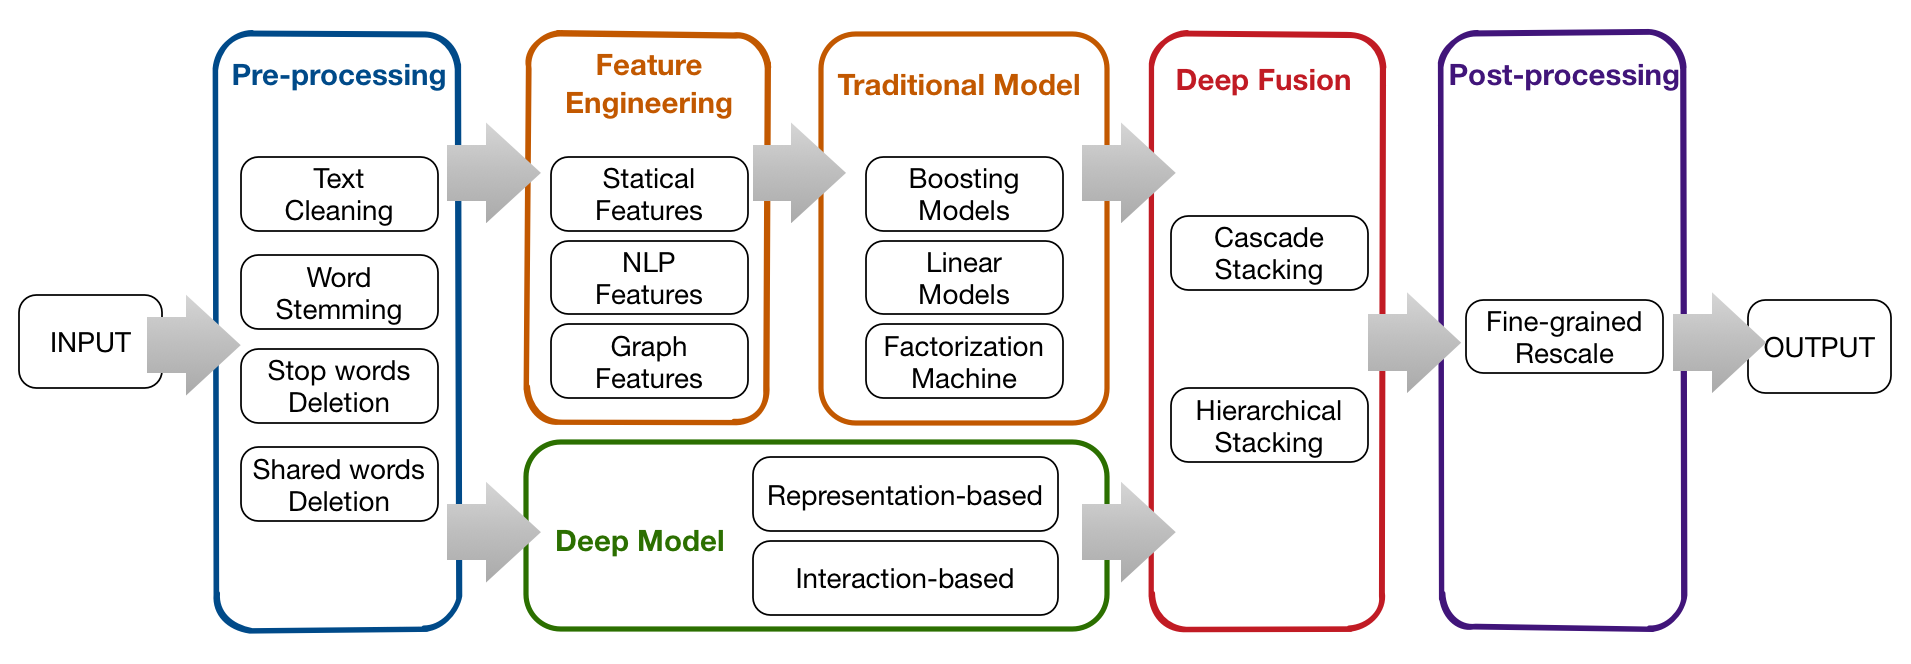
\includegraphics[width=0.9\textwidth]{../img/flowchart}\\
  \caption{The flowchart of our method.}
  \label{fig:Flowchart}
\end{figure}

\subsection{Submission}
\label{subsec:Results_description}

Submissions were evaluated on the log loss between the predicted values and the group truth. In specific, the best single model we have obtained during the competition was an XGBoost model with tree booster of Public LB score \textbf{0.12653} and Private LB score \textbf{0.13067} (without post-process). Our final submission was a stacking result of multiple models. This submission scored \textbf{0.11450} on Public LB and \textbf{0.11768} on Private LB (with post-process), ranking \textbf{4} out of \textbf{3396} teams.

\section{Pre-processing}


Pre-processing

\section{Feature Engineering}

Feature Engineering  

\section{Modeling}

\subsection{Data Partition}

Five-fold cross-validation is performed on this data set. In detail, the original training data set is randomly divided into five parts (S1-S5) each with approximately the same size. In each fold, one part is held-out for validation, another part is held-out for testing and the learning algorithm is trained on the remaining data. The above process is iterated five times so that each part is used as the validation data and test data exactly once, where the averaged metric values out of five runs are reported for the algorithm. Table~{\ref{tab:data-part-cv}} illustrates how to split the training data set for cross validation.

\begin{table}[ht]
\centering
\caption{Data Partition for Cross Validation}
    \label{tab:data-part-cv}
\begin{tabular}{p{3cm}p{3cm}p{3cm}p{3cm}}
\hline
 Fold & Training	& Validation        & Test \\
\hline\hline
Fold1 & S1, S2, S3 & S4 & S5 \\ \hline
Fold2	&	S2, S3, S4	&	S5	&		S1 \\ \hline	
Fold3	&	S3, S4, S5	&	S1	&		S2	\\ \hline
Fold4	&	S4, S5, S1	&	S2	&		S3	\\ \hline
Fold5	&	S5, S1, S2	&	S3	&		S4 \\ \hline
\end{tabular}
\end{table}

\section{Deep Fusion}

\subsection{Single Stacking}
\label{chap:single-stacking}

Stacking is a way of combining multiple models. The usual method for stacking is split the training set into two disjoint sets. Then train several base learners on the first part and test the base learners on the second part. Finally, using the predictions from second part as the input, and the correct responses as the output, train a higher level learner.

As you can see, the traditional stacking method use only part of the data to construct higher level learner. In order to use entire data while stacking, we proposed a novel way. The algorithm described as follows:

\begin{itemize}
\label{alg:single-stacking}
\item[1.] Randomly split offline data set into five subsets (5-fold CV for example).
\item[2.] Fit and make predictions based on this split with specified model 5 times: select 3 parts for training, 1 for validation and 1 for test every time.
\item[3.] Concat the prediction results on test data and use it as a new feature for offline data set.
\item[4.] Make prediction for online data 5 times with models generated in steps 2 and collect the results.
\item[5.] Random select a prediction result for every data points in online data set and form the new feature for online data set.
\item[6.] Using the new feature generated in steps 3 and 5 together with original features train a higher level learner and predict for online data set.
\end{itemize}

Alg.~{\ref{alg:single-stacking}} described how to stack a specified model into a higher level model. The flowchart of the Algorithm is shown in Fig.~{\ref{fig:single-stacking}}.


\begin{figure}[ht]
  \centering
  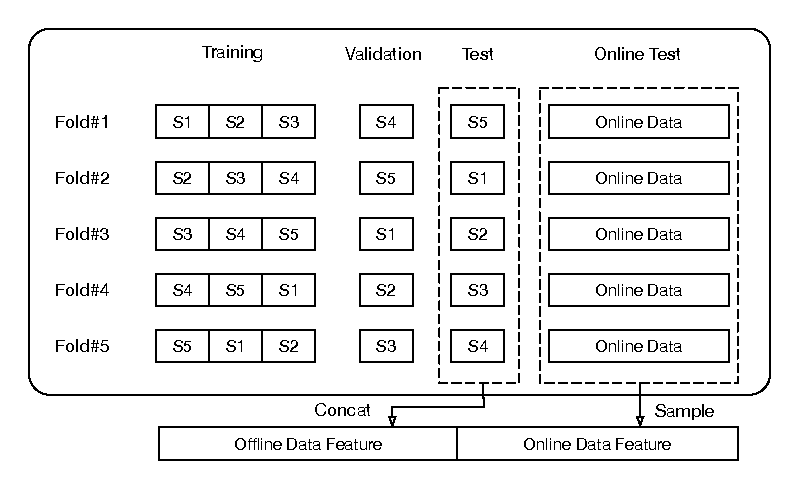
\includegraphics[width=0.8\textwidth]{../img/single-stacking}\\
  \caption{The flowchart of single stacking.}
  \label{fig:single-stacking}
\end{figure}

\subsection{Cascade Stacking}

With the single-stacking algorithm proposed in Chap.~{\ref{chap:single-stacking}}, we can construct a more complex stacking structure named Cascade Stacking. The framework of the Cascade Stacking is shown in Fig.~{\ref{fig:cascade-stacking}}. The steps of the cascade stacking described as follows:

\begin{itemize}
\label{alg:cascade-stacking}
\item[1.] Fit and make predictions based on original features with diverse models, such as XGBoost, LightGBM and Deep Models.
\item[2.] Convert the prediction results into new features through single-stacking algorithm.
\item[3.] Fit and make predictions based on all of the transformed features and original features with diverse models, such as XGBoost, LightGBM.
\item[4.] Fit and make predictions with Linear Regression Models based on all of the transformed features and without original features.
\item[5.] Repeat steps 3 and 4 until prediction score is converged.
\item[6.] Generate the final prediction result based on all of previous transformed features and original features with XGBoost.
\end{itemize}


\begin{figure}[ht]
  \centering
  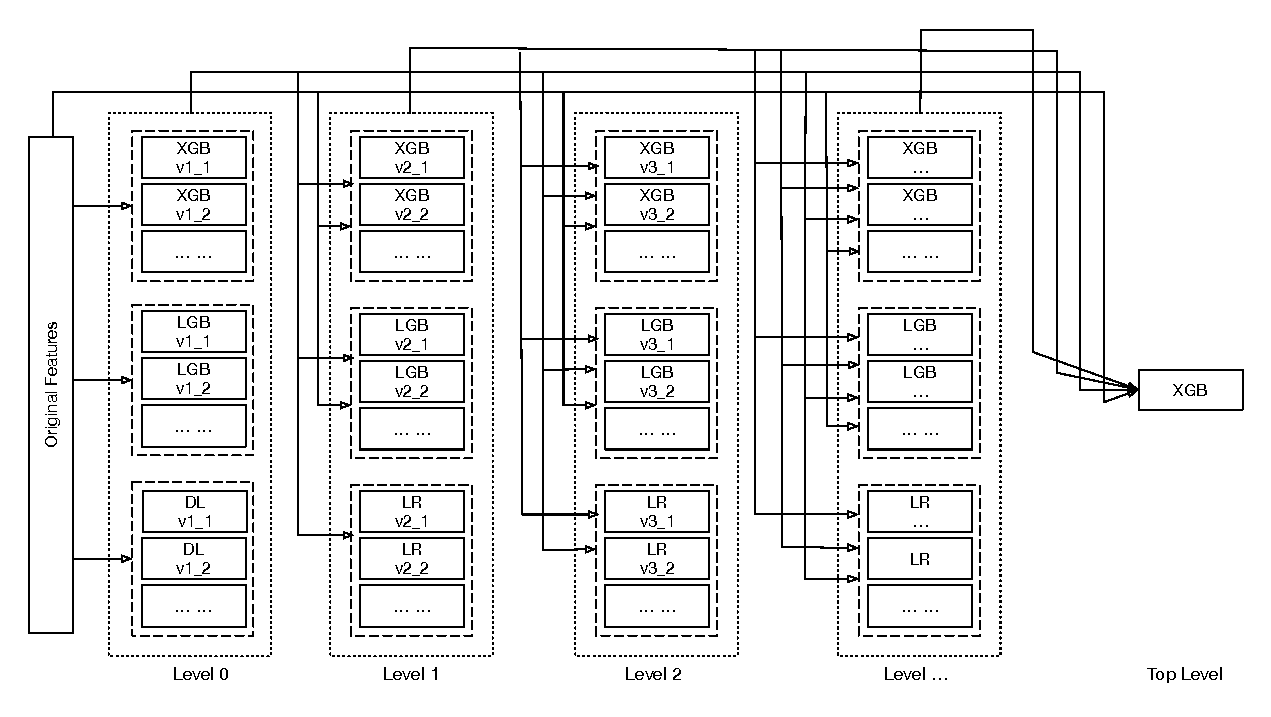
\includegraphics[width=1.0\textwidth]{../img/cascade-stacking}\\
  \caption{The framework of cascade stacking.}
  \label{fig:cascade-stacking}
\end{figure}

\subsection{Hierarchical Stacking}

Although Cascade Stacking method can improve the performance obviously compared to other stacking methods, it has some problems which are difficult to deal with:

\begin{itemize}
\item[1.] When the original features are increased, we must rebuild all of the models generated during cascade stacking from the bottom to the top. This rebuilding process is extremely time consuming.
\item[2.] During the number of layers increased gradually, the importance of the original features is reduced. The construction of the model is mainly based on the transformed features. 
\end{itemize}

In order to deal with those problems, we proposed another interesting structure of stacking named \textbf{Hierarchical Stacking}. The framework of the Hierarchical Stacking  is shown in Fig.~{\ref{fig:hierarchical-stacking}. The steps of the hierarchical stacking described as follows:

\begin{itemize}
\label{alg:cascade-stacking}
\item[1.] Fit and make predictions based on original features with diverse models, such as XGBoost, LightGBM and Deep Models.
\item[2.] Convert the prediction results into new features through single-stacking algorithm.
\item[3.] Fit and make predictions based on last layer transformed features and new extracted features with diverse models, such as XGBoost, LightGBM.
\item[4.] Fit and make predictions with Linear Regression Models based on last layer transformed features and without any original features.
\item[5.] Repeat steps 3 and 4 until prediction score is converged.
\item[6.] Generate the final prediction result based on last layer transformed features with XGBoost.
\end{itemize}


\begin{figure}[ht]
  \centering
  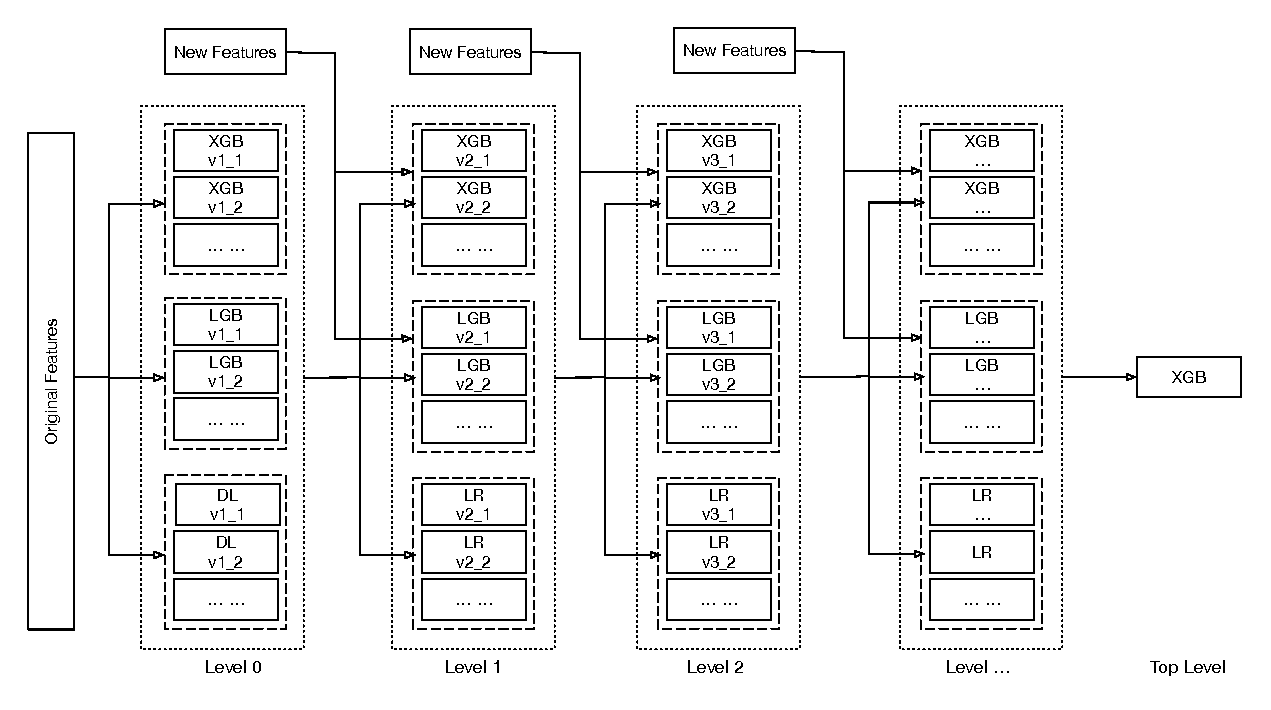
\includegraphics[width=1.0\textwidth]{../img/hierarchical-stacking}\\
  \caption{The framework of hierarchical stacking.}
  \label{fig:hierarchical-stacking}
\end{figure}

\section{Post-processing}

As the distribution of the offline data set (train.csv) and online data set (test.csv) are quite different, we did a post-processing procedure for the prediction results of online data set. We cut the data set into multiple sets according to the clique size and rescale the results in different parts separately.

\subsection{Split}

In order to reduce the impact of inconsistent between offline data set and online data set, we must split the data set into different parts. The standards of the division is the feature 'graph\_edge\_max\_clique\_size' and the feature 'graph\_edge\_cc\_size'. The meaning of the features is as follows:

\begin{itemize}
\item \textbf{graph\_edge\_max\_clique\_size} (mc\_size): Number of nodes contained in the largest clique of the edge.
\item \textbf{graph\_edge\_cc\_size} (cc\_size): Number of nodes contained in the connected component of the edge
\end{itemize}

With these features, we can divide the data set into four parts and the size of each part is described in Table~{\ref{tab:data-part-post}.

\begin{table}[ht]
\centering
\caption{Data Partition for Post-processing}
    \label{tab:data-part-post}
\begin{tabular}{p{2cm}cccc}
\hline
\multirow{2}*{}  & $mc\_size < 3$	& $mc\_size < 3$	& \multirow{2}*{$mc\_size = 3$}	&	\multirow{2}*{$mc\_size > 3$} \\
				&	$cc\_size < 3$	&	$cc\_size \geq 3$	&	&	\\
\hline\hline
train.csv & 118,065 & 173,164 & 40,482	&	72,579 \\ \hline
test.csv	&	1,933,597	&	344,283	&		23,841	&	44,075 \\ \hline
\end{tabular}
\end{table}

However, there are lots of fake data points in the online data set (test.csv). So the size of different parts for online data set is not true. We need to solve the nonlinear equations to obtain the true data ratio and positive samples ratio of different parts for online data.

Suppose the online data is cut into two parts. Let $k_1, k_2$ denote the data ratio of different parts for online data, and let $r_1, r_2$ be the positive samples ratio of different parts for online data. We can assigned the same value as prediction results for different parts $v_1, v_2$. Then we can get the $score$ back based on these values. In this way , you can get an equation as follows:

\begin{eqnarray}
k_1 * (r_1 * log(v_1) + (1 - r_1) * log(1 - v_1)) + k_2 * (r_2 * log(v_2) + (1 - r_2) * log(1 - v_2)) = - score
\label{eqn:pos_rate}
\end{eqnarray}

Then we can change the value of $v_1, v_2$ and can get the corresponding scores. Using those values, we can construct nonlinear equations. Based on equations, we will known the value of $k_1, k_2, r_1, r_2$.

In this competition, we have more variables to be solved and the solution is the same.

Finally, we get the data ratio and positive samples ratio of different parts for data sets. The data ratio is shown in Table~{\ref{tab:data-ratio}}. The positive samples ratio is shown in Table~{\ref{tab:pos-sample-ratio}}.

\begin{table}[ht]
\centering
\caption{Data Ratio of Different Parts}
    \label{tab:data-ratio}
\begin{tabular}{p{2cm}cccc}
\hline
\multirow{2}*{}  & $mc\_size < 3$	& $mc\_size < 3$	& \multirow{2}*{$mc\_size = 3$}	&	\multirow{2}*{$mc\_size > 3$} \\
				&	$cc\_size < 3$	&	$cc\_size \geq 3$	&	&	\\
\hline\hline
train.csv & 29.20\% & 42.83\% & 10.01\%	&	17.95\% \\ \hline
test.csv	&	30.50\%	&	52.19\%	&		6.08\%	&	11.24\% \\ \hline
\end{tabular}
\end{table}

\begin{table}[ht]
\centering
\caption{Positive Samples Ratio of Different Parts}
    \label{tab:pos-sample-ratio}
\begin{tabular}{p{2cm}cccc}
\hline
\multirow{2}*{}  & $mc\_size < 3$	& $mc\_size < 3$	& \multirow{2}*{$mc\_size = 3$}	&	\multirow{2}*{$mc\_size > 3$} \\
				&	$cc\_size < 3$	&	$cc\_size \geq 3$	&	&	\\
\hline\hline
train.csv & 23.35\% & 14.95\% & 62.32\%	&	97.26\% \\ \hline
test.csv	&	5.74\%	&	4.50\%	&		40.88\%	&	96.50\% \\ \hline
\end{tabular}
\end{table}

\subsection{Rescale}

As we get the positive samples ratio of different parts, we can rescale the prediction results in different parts seperately based on those prior knowledge.

For the specified part of data set, let $r_{offline}$ denote the positive samples rate on offline data set and let $r_{online}$ be the positive samples rate on online data set. The original values of prediction is $y$, then we can get the rescaled prediction values as follows:

\begin{eqnarray}
y_{rescale} = \frac{\frac{t_{test}}{t_{train}} * y}{\frac{t_{test}}{t_{train}} * y + \frac{1 - t_{test}}{1 - t_{train}} * (1 - y)}
\label{eqn:rescale_y}
\end{eqnarray}


\section{ML Framework}

We developed a light weight Machine Learning framework \textbf{FeatWheel} to help us finishing ML jobs, such as feature extraction, feature merging and so on. We will introduce the framework in this section.

\subsection{Characteristics}

\begin{itemize}
\label{list:characteristics}
\item \textbf{Simple}: With FeatWheel, you can focus on extracting features. All you need to do is to generate feature files in specified format and write a config file.
\item \textbf{Flexible}: You can specify the features you need and FeatWheel can help you finish the procedure of feature merging. You can also store the merging result on the disk to speed up the next loading process.
\item \textbf{Efficient}: If you want to split the data set into training, validation and test data, you just need to generate index files. You don't need make any changes to feature files and data set files.
\item \textbf{Reliable}: Each time of the model training and prediction will generate a separate output directory
\end{itemize}

\section{Acknowledgement}

Acknowledgement

\end{document}
